\documentclass[mathserif, 10pt]{beamer}
\usepackage[utf8]{inputenc}
\usepackage{amsmath, amsfonts}
\usepackage{appendixnumberbeamer}


\title{IFT Seminar, 27 January 2022}
\subtitle{Jorge Alda,\\ Universidad de Zaragoza/CAPA \hspace{4em} \texttt{jalda@unizar.es} }
\author[Jorge Alda]{Based on \textbf{JA}, J. Guasch, S. Peñaranda \\
arXiv:2109.07405 [hep-ph]}

\date[IFT Seminar]{IFT Seminar, 27th January 2022}



\usetheme{Zaragoza}
\usecolortheme{Unizar}
\titlepagelogoA{
\includegraphics[width=6cm]{logos/CAPA.png}}
\titlepagelogoB{
\includegraphics[width=4cm]{logos/dftuz2.png}}


\newcommand\colorcite[1]{{\scriptsize\color{blue}#1}}

\begin{document}
\begin{frame}[noframenumbering,plain]
\titlepage
\end{frame}

\begin{frame}
    \frametitle{$B$ anomalies}

    Experimental results for the decays of $B$ mesons that don't conform with the SM predictions.

    ~

    In particular, these anomalies show hints of violation of the Leptonic Flavour Universality (LFU)

\end{frame}

\begin{frame}
    \frametitle{$B$ anomalies}

    Flavour-changing neutral currents $b \to s \ell^+ \ell^-$, with $\ell = e, \mu$.
    \begin{itemize}
        \item Universality ratios $R_{K^{(*)}}$
              $$R_{K^{(*)}} = \frac{\mathrm{BR}(B\to K^{(*)}\mu^+ \mu^-)}{\mathrm{BR}(B\to K^{(*)}e^+ e^-)}\,, $$
              In the SM, theoretically clean, and $R_{K^{(*)}}=1$.\\
              LHCb measurements\footnote{arXiv:2103.11769, arXiv:1705.05802}:
              \begin{itemize}
                  \item $R_{K^+} = 0.846^{+0.042}_{-0.039}{}^{+0.013}_{-0.012}$,
                  \item $R_{K^{*0}} = 0.685^{+0.113}_{-0.069}\pm0.047$. ($3.1\,\sigma$ tension)
              \end{itemize}
        \item Angular observables for $B\to K^* \ell^+\ell^-$: $P'_4$, $P'_5$...
        \item Also $B_s \to \phi \mu^+ \mu^-$ decays.
    \end{itemize}

\end{frame}

\begin{frame}
    \frametitle{$B$ anomalies}
    Flavour-changing charged currents $b\to c \ell \nu$, with $\ell = e/\mu, \tau$.
    \begin{columns}
        \begin{column}{0.55\textwidth}

            \begin{itemize}
                \item Universality ratios $R_{D^{(*)}}$
                      $$R_{D^{(*)}} = \frac{\mathrm{BR}(B\to D^{(*)}\tau \nu)}{\mathrm{BR}(B\to D^{(*)}\ell \nu)}\,, $$
                      Combined tension of $3.08\,\sigma$.\footnotemark[1]
                \item Longitudinal polarization of $D^*$.
                \item Also $B_c \to J/\psi \ell\nu$ decays.
            \end{itemize}

        \end{column}
        \begin{column}{0.5\textwidth}
            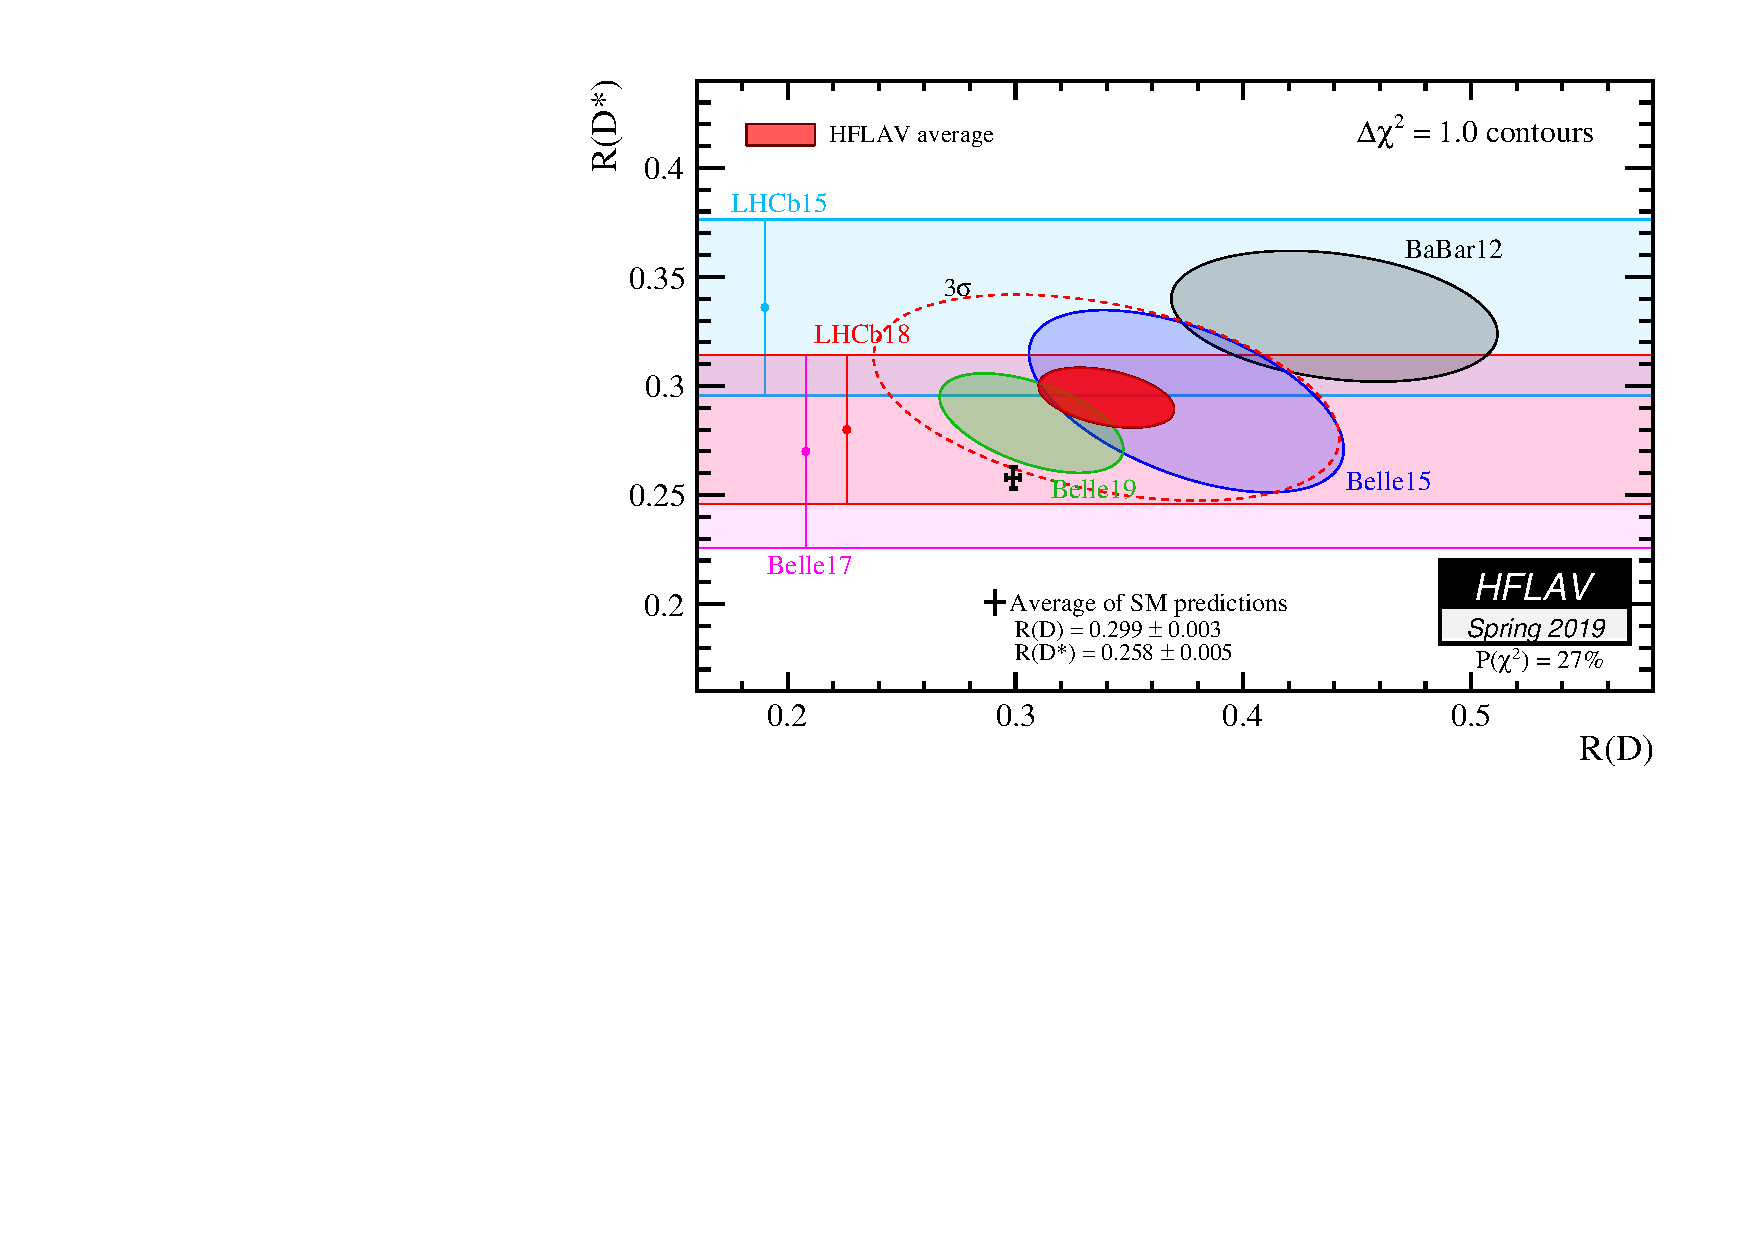
\includegraphics[width=\columnwidth]{figures/rdrds_spring2019.pdf}
        \end{column}
    \end{columns}
    \footnotetext[1]{arXiv:1909.12524}
\end{frame}

\begin{frame}
    \frametitle{Effective Field Theories}

    Effective Field Theories (EFTs) describe deviations from the SM in a model-independent way, using effective operators of dim $>4$ and their corresponding Wilson coefficients.

    ~

    At energies $\Lambda$ above the electroweak scale, the SMEFT (2499 operators)\footnote[1]{arXiv:1008.4884}

    $$\mathcal{L} = \mathcal{L}_\mathrm{SM} + \frac{1}{\Lambda^2}\sum C_i O_i\,.$$

    We will focus on the following operators at $\Lambda = 1\,\mathrm{TeV}$:

    $$O_{\ell q(1)}^{ijkl} = (\bar{\ell}_i \gamma_\mu \ell_j)(\bar{q}_k \gamma^\mu  q_l),\qquad\qquad O_{\ell q(3)}^{ijkl}= (\bar{\ell}_i \gamma_\mu \tau^I \ell_j)(\bar{q}_k \gamma^\mu \tau^I q_l)\,.$$

\end{frame}

\begin{frame}

    \frametitle{Effective Field Theories}
    The $B$ anomalies are defined at $\mu=m_b$, we need to integrate the heavy SM particles. We obtain the WET:

    ~

    \begin{itemize}
        \item $\left.\begin{matrix}
                      O_9^\ell = (\bar{s}_L \gamma_\alpha b_L)(\bar{e}_\ell \gamma^\alpha e_\ell) \\
                      O_{10}^\ell = (\bar{s}_L \gamma_\alpha b_L)(\bar{e}_\ell \gamma^\alpha \gamma_5 e_\ell)
                  \end{matrix}\right\} \qquad \Longrightarrow \qquad R_{K^{(*)}}$.

              ~

        \item $O_{VL}^\ell = (\bar{c}_L \gamma_\alpha b_L)(\bar{e}_{\ell\,L} \gamma^\alpha \nu_\ell) \qquad\Longrightarrow\qquad R_{D^{(*)}}$.

              ~

        \item $O_\nu^\ell = (\bar{s}_L \gamma_\alpha b_L)(\bar{\nu}_\ell (1-\gamma_5) \nu_\ell) \qquad\Longrightarrow \qquad \mathrm{BR}(B\to K^{(*)}\nu\overline{\nu})$.
    \end{itemize}



\end{frame}

\end{document}